\documentclass[german]{latex4ei/latex4ei_sheet}
\usepackage{stix}
\usepackage[ngerman]{babel} 
% set document information
\title{Hochfrequenztechnik \\ Cheat Sheet}
\author{Raoul Duke}
\myemail{0x4723@gmail.com}
\mywebsite{www.github.com/doppelplus/CheatSheets}

\begin{document}

\maketitle
\section{Allgemeines}
    \begin{sectionbox}
        \begin{bluebox}{Frequenz und Wellenlänge}
            \item Lichtgeschwindigkeit: $c = 299792458\,m/s$
            \item $F = \frac{c}{\lambda} \rightarrow \lambda = \frac{c}{F}$
        \end{bluebox}
    \end{sectionbox}

\section{(Wideband) Code Division Multiple Access}
    \begin{sectionbox}
        \begin{bluebox}{Signalspreizung}
            \item Direct Sequence CDMA.
            \item Datenstrom wird bei Sender \& Empfänger mit Spreizcode multipliziert.
            \item Mehrere Datenströme können im gleichen Frequenzband übertragen werden.
            \item 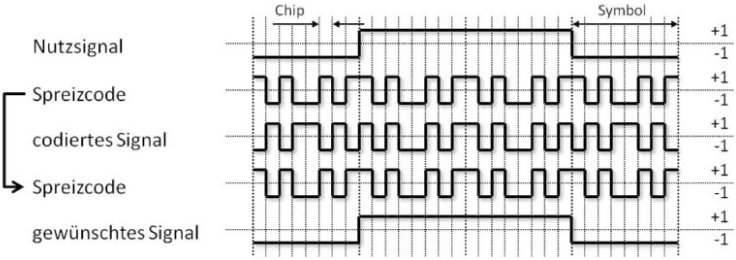
\includegraphics[width=185px]{img/Signalspreizung.png}
            \item Das Spektrum des gespreizten Nutzsignals ist um ein vielfaches breiter, als das originäre Signal. 
        \end{bluebox}
        \begin{symbolbox}{Formelzeichen}
            \item Spreizfaktor: $SF$
            \item Processing Gain: $PG$
            \item Chiprate: $b_c$
            \item Nutzdatenrate: $b_n$
            \item Störabstand: $SIR$
            \item Signalleistung: $S$
            \item Anzahl der aktiven Signale in der Funkzelle: $N$
            \item Mittlere Nutzenergie pro Bit: $E_b$
            \item Rauschenergie pro Bit: $N_0$
        \end{symbolbox}
        
        \begin{bluebox}
            \item $PG = 10\log SF\,dB$
            \item $SF = \frac{b_c}{b_n}$
            \item $SIR = \frac{S}{(N-1)\cdot S}= \frac{1}{1 N-1}$
            \item $\frac{E_b}{N_0} = \frac{S/b_N}{((N-1)S)/b_c} = \frac{1}{N-1}\cdot \frac{b_c}{b_N} = SIR \cdot SF$
            \item $10 \cdot \log \left(\frac{E_b}{N_0}\right) = 10\cdot \log (SIR)+ PG\,dB$
            \item $N = \frac{b_C}{E_b/N_0\cdot b_N}+1$
        \end{bluebox}
    \end{sectionbox}
\vspace{4cm}
    \section{Orthogonal Frequency Division Multiplexing}
    \begin{sectionbox}
        \begin{symbolbox}{Formelzeichen}
            \item Bandbreite: $W$
            \item Anzahl der Unterträger: $n$
            \item Breite der Unterträger: $B_U$+
            \item Symboldauer: $T_D$
            \item Zeitintervall: $T_S$ 
            \item Datensymbole: $D_0 \dots D_{-1}$
            \item Grundfrequenz: $f_G$
            \item Kanalfrequenz: $f_k$
            \item Abtastrate: $f_A$
        \end{symbolbox}
        
        \begin{bluebox}{Formeln}
            \item $B_U = \frac{W}{n}$
            \item $f_k =k \cdot f_G$\quad $k$ ganzzahlig mit $-\frac{n}{2}\geq k \geq \frac{n}{2}-1$ 
            \item $f_A = f_G = \frac{1}{T_S}$
            \item $T_S = n \cdot T_D$
            \item $\Delta f = f_k - f_{k-1} = k\cdot f_G -(k-1)\cdot f_G = f_G$
        \end{bluebox}
    \end{sectionbox}

    \section{Funkfelddämpfung}
    \begin{sectionbox}
        \begin{symbolbox}{Formelzeichen}
            \item 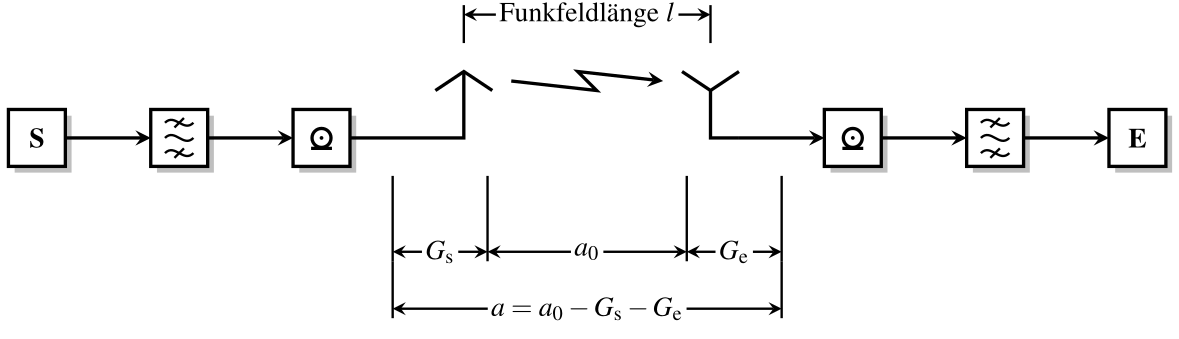
\includegraphics[width=185px]{img/Funkuebertragungssystem.png}
            \item Gewinn der Sendeantenne: $G_s$
            \item Gewinn der Empfangsantenne: $G_e$
            \item Sendeleistung: $P_s$
            \item Empfangsleistung: $P_e$
            \item Funkfelddämpfung: $a$
            \item Freiraumdämpfung: $a_0$
        \end{symbolbox}
        
        \begin{bluebox}{Formeln}
            \item $a = \frac{P_s}{P_e} = \frac{(4\pi l)^2}{\lambda^2 G_e G_s}$ \textbf{als Faktor}.
            \item $a = P_s - P_e = 20\lg \frac{4\pi l}{\lambda}-G_s-G_e$ \textbf{in dB}.
            \item $a_0 = 20\lg \frac{4\pi l}{\lambda}$
        \end{bluebox}
    \end{sectionbox}


\end{document}